\section{Dynamic Obstacles in a GridWorld} 
\label{gridworlddyn}
We first evaluate the performance of our \dio{}/rl implementation compared to an implementation making only use of reinforcement learning. 
We precisely look at (1) frames per second to evaluate speed. A \gls{frame} is a the step taken by the agent at one unit of time. Thus, frames/second 
during training are equivalent to how fast the learning takes. We also look at the mean of frames per episode and the mean of returns per episode to evaluate 
optimality. An \gls{episode} is defined as the collection of steps before we reach a terminal state, either 
through fatalities (e.g. colliding with an obstacle), goals or reaching the maximum number of steps that we set to 256 steps.
Finally, \glspl{return} is equivalent to a discounted summation of rewards. 
\subsection{Scenario in Reinforcement Learning}

Our autonomous agent exists in an 8x8 grid world. Its goal is to reach
the lower right position (8,8) from his initial position (1,1).
Along the way, there exists dynamic obstacles whose movements is
unknown. The agent is punished if colliding with an obstacle and the
\gls{episode}, hereby ends. 
This environment offered by gym-gridworld~\cite{gym_minigrid} is useful for testing our algorithm in a Dynamic Obstacle avoidance for a partially observable 
environment. Precisely, we define the state as follows. 
\begin{equation*}
  S_t = [x, y, d, G]
\end{equation*}
$(x,y)$ define the position of our agent while $d$ its direction. $G$
is the gridworld observed by the agent which includes walls, obstacles
and free squares. Note that this observed environment is from the point of the view 
of the agent and does not represent the entire grid. 
The action space is, 
\begin{equation*}
  A_t = \{ right: 0, up: 1, down: 2, left: 3 \}
\end{equation*}
Finally, the reward is a function of the distance from the goal
defined as, 
\begin{equation*}
  R_t = 1 - 0.9*(\dfrac{steps}{max\_steps})
\end{equation*}
Note that the $max_steps$ is defined by the manhattan distance between the agent and the goal. The intuition is 
we want to reward the agent the faster it reaches the goal. Additionally, the agent is punished with $-1$ if it collides with 
an obstacle, to encourage staying away from the dynamic obstacles. 
\newpage

\begin{multicols}{2}[\medskip]
    \begin{figure}[H]
      \centering
      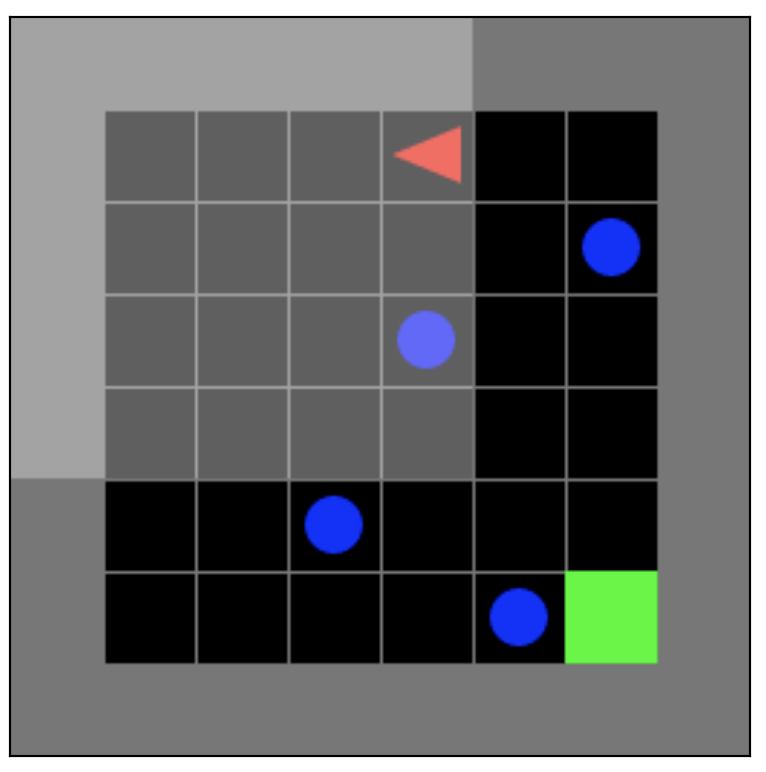
\includegraphics[scale=0.55]{figures/gridworldrl.png}
      \caption{Gridworld with Dynamic Obstacles}
      \label{fig:gridrl}
    \end{figure}
    \columnbreak
    The Reinforcement Learning experiments have been performed on 80k 
    episodes for a similar start configuration as shown in Figure~\ref{fig:gridrl}. The episode ends when the agent 
    reaches the goal \textbf{or} collides with an obstacle \textbf{or} reaches the maximum number of steps which is $256$. We want to encourage the shortest and safest path, thus, the punishment for crashing is $r = -1$. 
\end{multicols}

\subsection{Domain Specific Rules}
The rules are defined as a ProbLog~\cite{problog}: a probabilistic prolog that allows us to capture 
the stochasticity of the environment, as we previously introduced in \ref{sec:problog}. Precisely, we want to consider the erratic movements of the obstacles, considering 
we do not have previous knowledge on the distribution of their given movement. We assume a uniform distribution and define the following. 
The rules of \dio{} take the following form: 

\begin{prooftree}
  \AxiomC{$p_1 \dots p_n$}
  \AxiomC{$\sum_{i=0}^{n}P(i) = 1$}
  \RightLabel{(action)}
  \BinaryInfC{$P_i :: \varphi(i)$}
\end{prooftree}
We define $\sum_{i=0}^{n}P(i) = 1$, and $\varphi(i)$ corresponds to the conjunction of grounds facts of the possible world with probability $P_i$.
The action is equivalent to our step semantics, thus, we enforce that a given action modifies the facts in some form. In practice, an action is the missing 
clause to generate the next predicate. In the gridworld example, we give the following. 

\begin{multicols}{2}
\begin{prooftree}
  \AxiomC{atPos(X + V*T, Y)}
  \RightLabel{(right)}
  \LeftLabel{(1)}
  \UnaryInfC{atPos(X,Y), speed(V), timestep(T)}
\end{prooftree}
\columnbreak 
\begin{prooftree}
  \AxiomC{0.25 :: obs(X + V*T, Y, V) \ldots}
  \LeftLabel{(2)}
  \RightLabel{(time)}
  \UnaryInfC{obs(X,Y,V), timestep(T)}
\end{prooftree}
\end{multicols}

(1) considers the movement of the agent while (2) considers the movement of the obstacles. Note that (2) considers 
a uniform distribution over the movement of the obstacle, since every obstacle has a uniform probability of moving up/down/left/right. 
We could do the same for (1) by consider the probability of an action failing. In our case, we assume the movement is deterministic and no failure over the movement 
of the agent happens.


\subsection{World Knowledge}
Our world knowledge base covers the agent, the obstacles and the timestep. We consider two cases: 
\textit{constant} ground facts vs. \textit{dynamic} ground facts. The latter represents positions which are dynamically 
generated at every timestep while the former considers only the facts that remain true in every world, thus include the timestep, since we always
move by 1-unit, and the speed, since the agent and the obtacles are defined to only move by 1-box every time. Given that our knowledge base $Kb$ is defined by, 
\[
    C = \{speed(1), timestep(1) \}     
    \qquad
    D = \{atPos(X, Y), obs(X,Y,1)\}
    \qquad
    Kb = C \cup D
\]

\subsection{From Norms to Labels}
In the following, we define \textbf{\glsplural{norms}} as textual sentences to describe the intended goal behavior. 
Thus, in the gridworld example, we consider three possibles norms, (1) \textit{crash} when the agent and the obstacle overlap, (2) \textit{maybecrash} 
when the agent and the obstacle are one square from each other and finally (3) \textit{safe} when there is ample distance between the agent the obstacle 
in this case, two square distances. Those norms are identified as 'labels', i.e. predicates defined as follows. 

\[
    \infer{1 :: crash}{1 :: atPos(X,Y) & 1 :: obs(X,Y,\_)} 
    \qquad
    \infer{P_1 \times P_2 :: maybecrash}{P_1::atPos(X,Y), P_2::obs(X,Y,\_)
      & \ldots}
\] 
\[
    \infer{P_1 \times P_2 :: safe}{
      P_1::atPos(X_1,Y_1) & P_2::obs(X_2,Y_2,\_) & X_1 \neq X_2 & Y_1 \neq Y_2
      & \ldots
    }
\]
\[
  \infer{1.0/(L+T) :: close}{
    \_:nextPos(X,Y) & \_:goal(I,J) & \_:time(T) & L = abs(I-X) + abs(Y-J)
  }
\]

 \paragraph{Nondeterminism} 
 If we look at crash and maybecrash predicates, we notice that the two hold for the 
 same premises. This is what we define as non-determinism, where any of the two can be chosen. 
 The choice was made considering that a crash would imply a 'maybecrash', thus trivially true. 

\subsection{Translation Unit}
The translation unit is the bridge between \dio{} and RL. Precisely, it handles both feeding 
the world facts to \dio{} and translates the feedback given to a numerical value, through 
a given function. First, the \dio{}/RL loop is given in Algorithm 1. 

  \begin{algorithm}[H]
    \caption{\dio{}/RL Loop}
    \begin{algorithmic}[1]
    
    \Procedure{Step}{$S_t, a$}       \Comment{(State, action) Pair}
        \State Check for invalid actions
        \State Check for obstacles 
        \State Update Obstacles positions
        \State Update Agent's position
        \State \textbf{TU.UpdateWorld}(position, direction, obstacles) \Comment{KB update in \dio{}}
        \State $obs, reward$ = Step'$(S_t, ac)$ \Comment{Call to Initial Env}
        \State $J$ = \textbf{getFeedback()} \Comment{Query \dio{}}
        \State $reward$ = TU.getReward($J$) 
        \State return (obs,reward)
    \EndProcedure
    
    \end{algorithmic}
    \end{algorithm}

When it comes to reward shaping, we focus on the 'getFeedback' function. First, the translation units gets 
the labels, i.e. the probabilities of the evaluated predicates and constructs a function that associates 
every predicate to its corresponding numerical value. Finally, the reward is equivalent to weighted probabilities 
as shown in Algorithm 2, this is because of our \emph{design choice} to make our judgment as a numerical value. 
Trivially, the \textsc{getReward} from TU is an identity function.

\begin{algorithm}[H]
  \caption{Inference of Judgment $J$}
  \begin{algorithmic}[1]
      
      \Procedure{getFeedback}{} 
      \State labels $\gets$ \textbf{getLabels()} \Comment{Evaluated predicates w/ Corresponding Probabilities}
      \State $P \gets \{$crash, maybecrash, safe$\}$  \Comment{Set of possible worlds}
      \State $F \gets \{-1,-0.5,1\}$ \Comment{Numerical value associated with world}
      \State $i \gets 1$
      \State $r \gets 0$
      \While{$i \leq$ length(labels)} 
         \State $r \gets r +$ labels[P[i]]*F[i] \Comment{Equivalent to weighted probabilities}
         \State $i \gets i+1$


      \EndWhile
      
      \EndProcedure
      
      \end{algorithmic}
      \end{algorithm}

    \subsection{Results}
    Our testing was done on a Dynamic Obstacles grid world using proximal policy optimization over 80k frames. 
    We pick up the frames per second to evaluate the speed of learning, the mean number of frames per episode 
    to evaluate the optimality of the solution and finally, the mean returns per episode to evaluate convergence relative 
    to the number of frames. The code is available on github \cite{dio} with steps on how to replicate our model. 
    Refer to the beginning of \ref{gridworlddyn} for an explanation of the metrics. 

    \vspace{1cm}

    
    \begin{minipage}{.4\textwidth}  
      \centering 
      \textsc{DIO $+$ RL}
    \end{minipage}%
    \begin{minipage}{.4\textwidth}
      \centering
      \text{RL}
    \end{minipage}

    \begin{figure}[H]
      \centering
      \begin{minipage}{.4\textwidth}
        \centering
        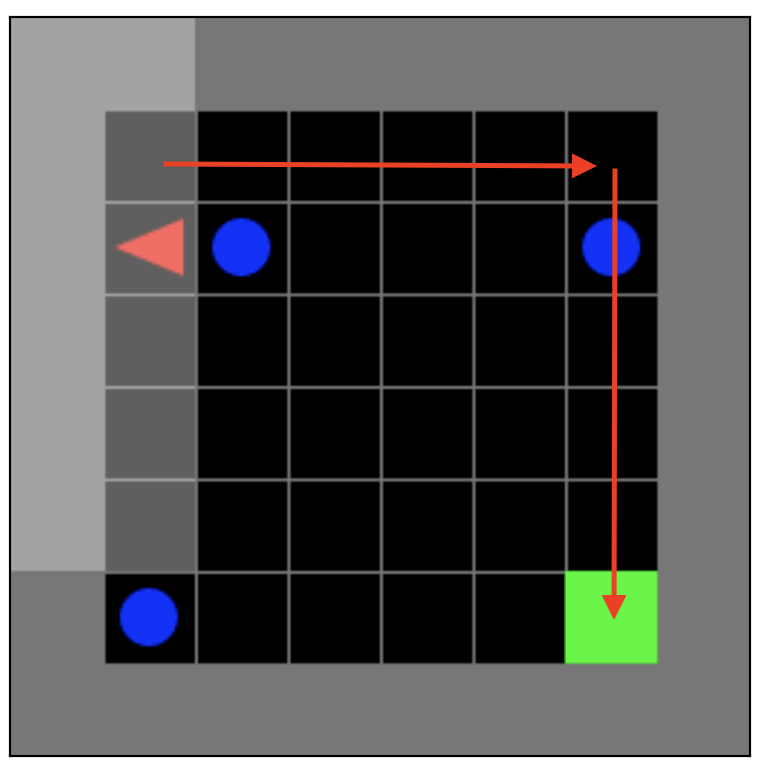
\includegraphics[width=1\linewidth]{figures/diopolicy.png}
        \captionof{figure}{\Gls{policy} learned with \dio{}}
        \label{fig:policydio}
      \end{minipage}%
      \begin{minipage}{.4\textwidth}
        \centering
        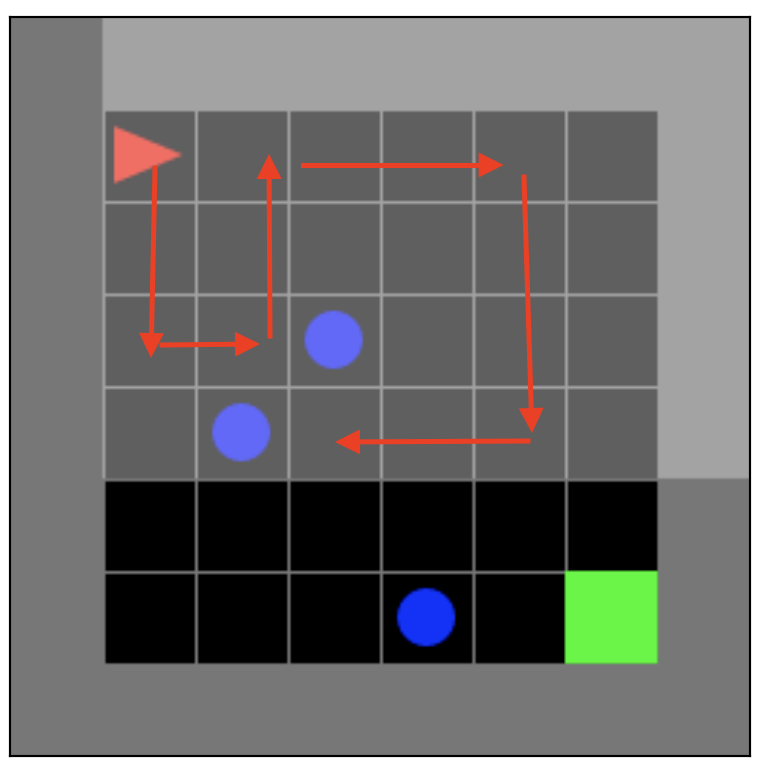
\includegraphics[width=1\linewidth]{figures/rlpolicy.png}
        \captionof{figure}{Policy learned without \dio{}}
        \label{fig:policyrl}
      \end{minipage}
    \end{figure}


    \begin{figure}[H]
      \centering
      \begin{minipage}{.5\textwidth}
        \centering
        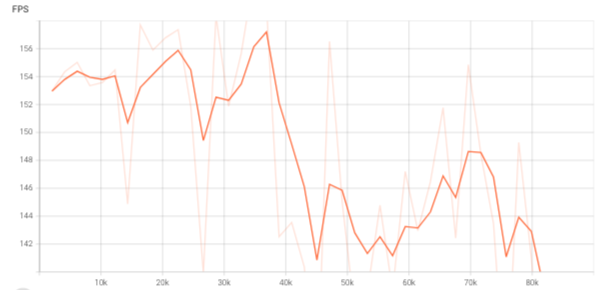
\includegraphics[width=1\linewidth]{figures/diofps.png}
        \captionof{figure}{Frames per Second with \dio{}}
        \label{fig:fpsdio}
      \end{minipage}%
      \begin{minipage}{.5\textwidth}
        \centering
        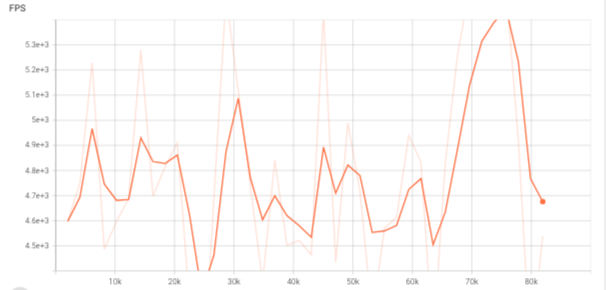
\includegraphics[width=1\linewidth]{figures/rlfps.png}
        \captionof{figure}{Frames per Second without \dio{}}
        \label{fig:fpsrl}
      \end{minipage}
    \end{figure}


    \begin{figure}[H]
      \centering
      \begin{minipage}{.5\textwidth}
        \centering
        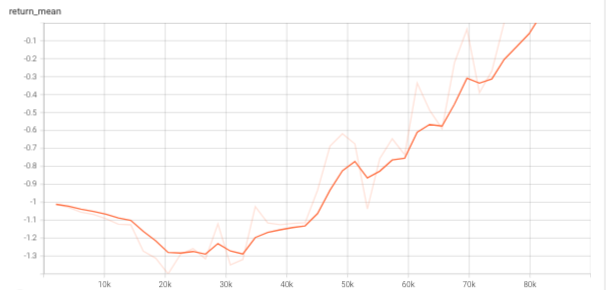
\includegraphics[width=1\linewidth]{figures/dioreturn.png}
        \captionof{figure}{Mean of \glspl{return} per episode with \dio{}}
        \label{fig:returndio}
      \end{minipage}%
      \begin{minipage}{.5\textwidth}
        \centering
        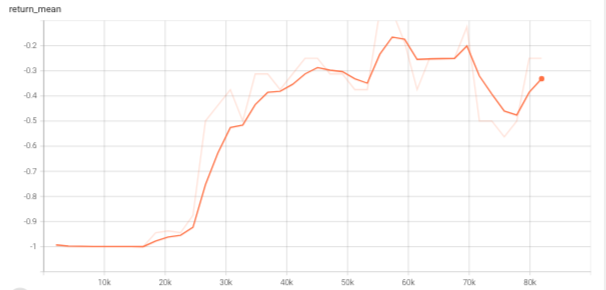
\includegraphics[width=1\linewidth]{figures/rlreturn.png}
        \captionof{figure}{Mean of returns per episode without \dio{}}
        \label{fig:returnrl}
      \end{minipage}
    \end{figure}

    \begin{figure}[H]
      \centering
      \begin{minipage}{.5\textwidth}
        \centering
        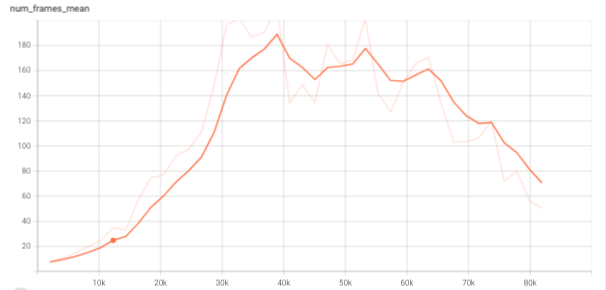
\includegraphics[width=1\linewidth]{figures/dioframesmean.png}
        \captionof{figure}{Mean of \glspl{frame} per episode with \dio{}}
        \label{fig:framesdio}
      \end{minipage}%
      \begin{minipage}{.5\textwidth}
        \centering
        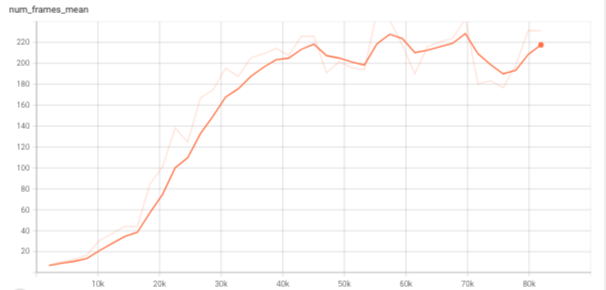
\includegraphics[width=1\linewidth]{figures/rlframesmean.png}
        \captionof{figure}{Mean of frames per episode without \dio{}}
        \label{fig:framesrl}
      \end{minipage}
    \end{figure}

    %%
    \paragraph{}
    We first visualized the learned policy in the two implementations. Althrough both learned 
    how to not crash into the Dynamic Obstacles, the implementation with \dio{} was better at minimizing the number of steps 
    but also learned to reach the goal. 

    %%
    \paragraph{}
    First, as expected, the implementation using \dio{} is much slower only able to run 
    an average of 150 episodes per second. As a result, for 80k episodes, the implementation with \dio{} 
    took 9 minutes to train versus 16 seconds for the implementation without. However, this loss in time shows as in \ref{fig:framesdio} 
    a gain in optimality. When visualizing the learned policy of \dio{}, we found that our agent succeeds in 90\% 
    of the time to reach the goal without colliding taking an average of $50 \pm 21$. Consider that 
    the optimal number of steps without obstacles is 13, while the policy learned without \dio{} did not reach a suitable solution and collides with an obstacle $17\%$ of the episodes. Furthermore, it takes an average of $231 \pm 59$ to end an episode 
    indicating that more than not, it ends the episode without ever reaching the goal. 


    %%
    \paragraph{}
    The dip in the mean frames in \ref{fig:framesdio} show that the agent did not only learn 
    how to only collide but also is learning how to reach the goal in the shortest amount of time. 
    Since \ref{fig:returndio} is still increasing, we can also tell that the values did not converge yet and 
    the agent can learn even a better optimization while \ref{fig:returnrl} shows that the values converge towards
    a suboptimal policy.


    \paragraph{}
    In \ref{fig:returndio} and \ref{fig:returnrl}, it is evident that the policy learned by \dio{} 
    is more optimal. Similarly, when evaluating our policies on the same reward scheme, 
    the implementation with \dio{} averages a 0.64 while without \dio{} averages a -0.18 return.

    %%
    \paragraph{}
    Overall, the results show that an implementation that makes use of
    \dio{} is beneficial even in a stochastic environment. As we lose in speed, we gain in optimality of the solution. 
    Given those preliminary results, we want to (1) optimize our implementation 
    and (2) test our implementation in a more complex scenario that requires a more complex understanding of the world 
    from \dio{} side. (1) is discussed in \ref{optimality} and (2) is discussed in \ref{traffic}. 

    
